\documentclass[../main-v1.tex]{subfiles}
\begin{document}
\chapter{Overview of the Computing Model \hideme{Anne comments addressed}}
\label{ch:cm}

%%%%%%%%%%%%%%%%%%%%%%%%%%%%%%%
\section{Introduction \hideme{JZ /anne comments 4/27}}\label{ch:cm:intro} %\hideme{Schellman/McNab -needed}}
% Need a proper name

%SURF -> FNAL -> off site storage -> processing -> analysis

%Simulation -> storage -> analysis




The current DUNE global computing model is an organic extension of the \dword{fnal} \dword{fife} computing model, used for smaller Intensity Frontier experiments, to the full global DUNE collaboration.  This effort  has relied heavily on global infrastructure such as \dword{osg} and the \dword{wlcg} and was successful for the first small-scale \dword{protodune} tests. However, it needs substantial enhancement to cope with the anticipated data and processing volumes.  This chapter describes the current situation and proposals for future improvements. 

\subsection{Global Resources}\label{model:global}

\dshort{dune} is a global collaboration  with contributions from institutions worldwide.   The long-term strategy for computing resources is for primary raw data storage to reside at the large host labs (the \dword{cern} and \dword{fnal}) with computing resources such as %disk and CPU 
CPU and storage largely contributed by collaborating %countries. 
institutions. CPU contributions are provided by a large number of sites worldwide as shown in Figure~\ref{fig:prodsites}, while storage is concentrated at a few larger %international 
sites. Table~\ref{tab:coop:disk} shows the distribution of disk space pledges for 2021 and 2022, while Tables~\ref{tab:coop:sites} and~\ref{tab:coop:ussites} list the sites contributing CPU resources. 

%HMS this was throwing errors. Also extended the caption. 
\begin{dunefigure}
[Wall time distribution of Production jobs FY22]
{fig:prodsites}
{Distribution of wall time for DUNE production jobs, October 2021 to March 2022. Inner ring: country. Outer ring: site. Over 50\% of wall hours have come from outside the United States in Fiscal Year 2022.}
{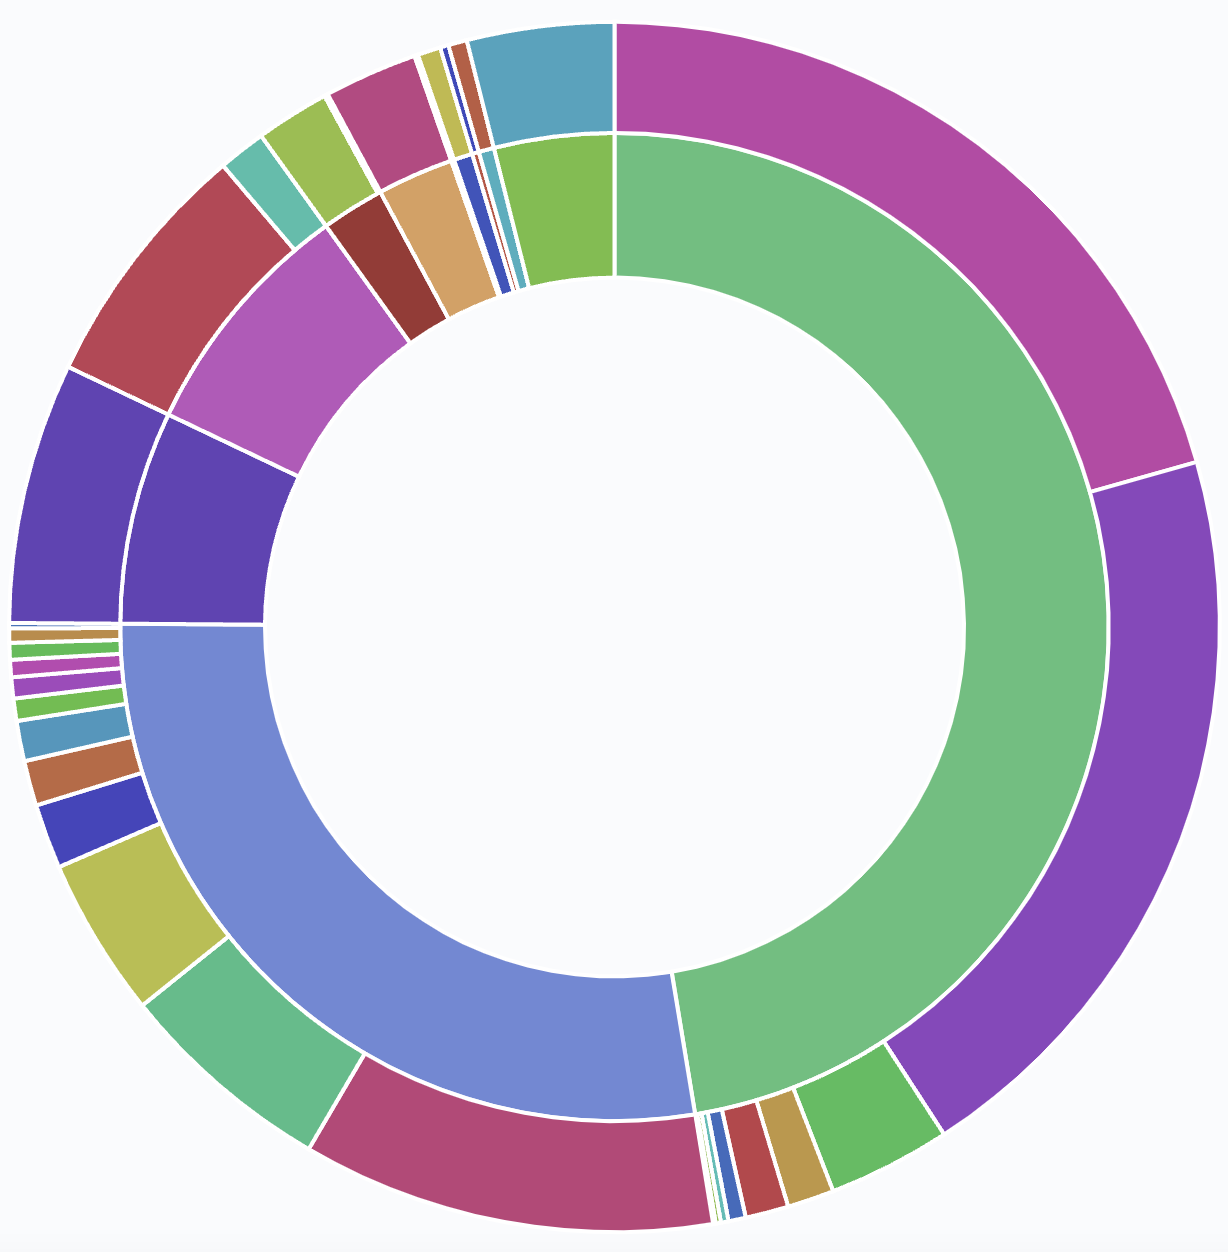
\includegraphics[height=3.5in,width=0.5\textwidth]{graphics/Workflow/walltimeplot.png}
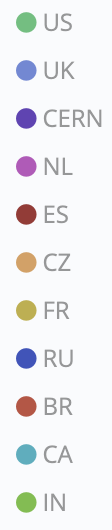
\includegraphics[height=3.5in,width=0.12\textwidth]{graphics/Workflow/walltimecountry.png}
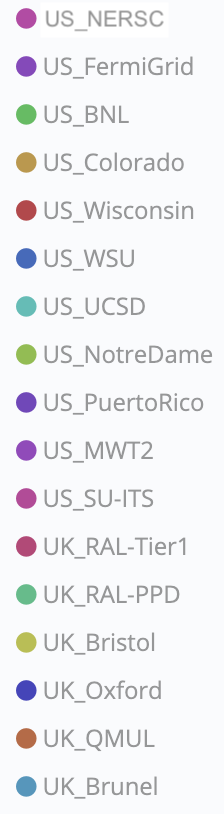
\includegraphics[height=3.5in,width=0.15\textwidth]{graphics/Workflow/walltimesite1.png}
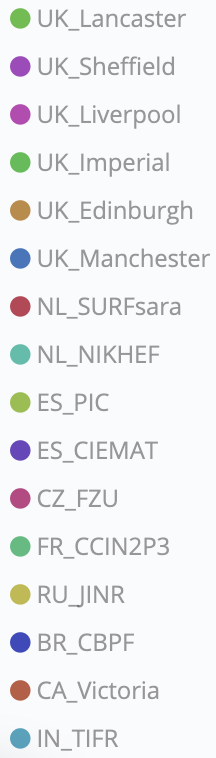
\includegraphics[height=3.5in,width=0.15\textwidth]{graphics/Workflow/walltimesite2.png}}
\end{dunefigure}

%This model builds on the highly successful tools developed by the WLCG and OSG for LHC computing.  As DUNE's needs are substantially smaller that those of the large LHC experiments we can be confident that the existing infrastructure can be incrementally augmented to meet DUNE's requirements. 

%\section{Current Global Computing Model}
%\todo{HMS done  Must update pledges}

\begin{dunetable}
[National disk pledges]{llrr}{tab:coop:disk}
{Disk pledges in PB for 2021 and 2022.}
Country/Lab	&	Name	&	2021	&	2022	\\
\dword{fnal}	&	\dword{fnal}	&	2.2	&	7.6	\\
\dword{cern}	&	\dword{cern}	&	2.2	&	3.0	\\
\dword{bnl}	&	\dword{bnl}	&	0.5	&	0.5	\\
United Kingdom	&	GridPP	&	4.0	&	4.0	\\
France	&	CC-IN2P3	&	0.5	&	0.5	\\
Spain	&	PIC Tier-1	&	0.5	&	0.72	\\
Netherlands	&	NL/LHC Tier-1	&	1.9	&	1.8	\\
Czechia	&	CZ-Prague-T2	&	0.3	&	1.0	\\
%BR	&	CBPF	&	0	&		\\
India	&	TIFR	&	0.75&	0.75\\
Russian Federation	&	JINR	&	-	&	0.5	\\
\hline
Total pledge	&		&	12.85	&	18.97	\\
Total request & & 20.4 & 27.3 \\
\end{dunetable}



%\tiny
\begin{dunetable}
[List of DUNE Compute Sites]
{l l r l}{tab:coop:sites}
{List of non-US international DUNE compute sites as of December 2021.  Sites with substantial \dword{rucio} controlled disk are noted.}
Site name	&	RC Site	&	Disk	&	Country	\\
\hline
BR\_CBPF	&	BR\_CBPF	&		&	Brazil\\
BR\_UNICAMP	&BR\_UNICAMP	&		&	Brazil\\
CA\_Victoria	&	CA\_Victoria	&		&	Canada\\
CERN	&	CERN-PROD	&	Yes	&	Switzerland\\
CH\_UNIBE-LHEP	&	UNIBE-LHEP	&		&	Switzerland\\
CZ\_FZU	&	FZU	&	Yes	&	Czechia\\
ES\_CIEMAT	&	CIEMAT-LCG2	&		&	Spain\\
ES\_PIC	&	pic	&	Yes	&	Spain\\
FR\_CCIN2P3	&	IN2P3-CC	&	Yes	&	France\\
IN\_TIFR	&	IN\_TIFR	&	Yes	&	India\\
NL\_NIKHEF	&	NIKHEF-ELPROD	&		&	Netherlands\\
NL\_SURFsara	&	SURFsara	&	Yes	&	Netherlands\\
RU\_JINR	&	JINR\_CONDOR\_CE	&	Yes	&	Russian Federation\\
UK\_Bristol	&	UKI-SOUTHGRID-BRIS-HEP	&		&	United Kingdom\\
UK\_Brunel	&	UKI-LT2-Brunel	&		&	United Kingdom\\
UK\_Edinburgh	&	UKI-SCOTGRID-ECDF	&		&	United Kingdom\\
UK\_Imperial	&	UKI-LT2-IC-HEP	&		&	United Kingdom\\
UK\_Lancaster	&	UKI-NORTHGRID-LANCS-HEP	&	Yes	&	United Kingdom\\
UK\_Liverpool	&	UKI-NORTHGRID-LIV-HEP	&		&	United Kingdom\\
UK\_Manchester	&	UKI-NORTHGRID-MAN-HEP	&	Yes	&	United Kingdom\\
UK\_Oxford	&	UKI-SOUTHGRID-OX-HEP	&		&	United Kingdom\\
UK\_QMUL	&	UKI-LT2-QMUL	&	Yes	&	United Kingdom\\
UK\_RAL-PPD	&	UKI-SOUTHGRID-RALPP	&		&	United Kingdom\\
UK\_RAL-Tier1	&	RAL-LCG2	&	Yes	&	United Kingdom\\
UK\_Sheffield	&	UKI-NORTHGRID-SHEF-HEP	&		&	United Kingdom\\

\end{dunetable}


\begin{dunetable}
[List of US DUNE Compute Sites]
{l l r }{tab:coop:ussites}
{List of US DUNE compute sites as of December 2021.  Sites with substantial rucio controlled disk are noted.}
US\_UConn-HPC	&	UConn-HPC	&	Disk\\
US\_BNL	&	BNL-SDCC-CE01	&	Yes	\\
US\_Caltech	&	CIT\_CMS\_T2	&	\\
US\_Clemson	&	Clemson-Palmetto	&	\\
US\_Colorado	&	UColorado\_HEP	&	\\
US\_Florida	&	UFlorida-HPC	&	\\
US\_FNAL	&	GPGrid	&	Yes	\\
US\_KSU	&	BEOCAT-SLATE	&	\\
US\_Lincoln	&	Rhino	&	\\
US\_Michigan	&	AGLT2	&	\\
US\_MIT	&	MIT\_CMS	&		\\
US\_MWT2	&	MWT2	&		\\
US\_Nebraska	&	Nebraska	&	\\
US\_NERSC & NERSC &   \\
US\_NMSU-DISCOVERY	&	SLATE\_US\_NMSU\_DISCOVERY	&	\\
US\_NotreDame	&	NWICG\_NDCMS	&	\\
US\_Omaha	&	Crane	&	\\
US\_PuertoRico	&	uprm-cms	&	\\
US\_SU-ITS	&	SU-ITS-CE2	&	\\
US\_UChicago	&	MWT2	&	\\
US\_UCSD	&	UCSDT2	&	\\
US\_Wisconsin	&	GLOW	&	\\
US\_WSU	&	WSU - GRID\_ce2	&	\\
\end{dunetable}


%anne 3/15 \section{Site characteristics}

%\fixme{add a section which describes the various site types - HPS, normal, analysis, commercial services - I think this is already done in section 6.4 - Kirby (anne removed section header)}
%\todo{Add diagrams}

Computing resources are currently dominated by conventional unix batch systems accessible via the \dword{osg} and \dword{wlcg} but HPC resource such as \dword{nersc} and commercial resources such as GPUs from Google Cloud\cite{Wang:2020fjr} are also being tested and used when useful and available. 

\dword{dune}'s model is flatter and more network oriented than the original model for \dword{lhc} experiments.   As a result, it relies mainly on well connected data centers for storage and \dword{cpu} provision.  To date, we have found that most users prefer to do their work through the large national facilities available to them rather than building and using small local clusters at their home institutions.  


\section{Current Performance}\label{ch:model:perf} %\hideme{Schellman/Herner - draft}}. 

\dshort{dune} has performed multiple simulation and reconstruction passes on the \dword{pdsp} data and is running significant simulation campaigns for the \dword{fd} and \dword{nd} design and physics studies. The \dword{poms} and \dword{sam} described in Chapters~\ref{ch:datamgmt} and~\ref{ch:wkflow}, are highly instrumented and allow assessments of the performance of the global computing system in near-real time.  There are four major data/CPU access patterns:
\begin{itemize}
    \item Simulation requires little input (mainly beam flux files and photon libraries),  has a large memory footprint, uses significant CPU resources and writes back a few large files.
    \item Hit reconstruction and pattern recognition both read in large files, have an intermediate memory footprint and uses $\sim$10\,sec/MB of input data.  
    \item Data reduction reads the reconstructed data and produces small tuple outputs for further analysis.  Reduction uses $\sim0.1$\,sec/MB of input data and is generally IO limited.
    \item Data analysis consists of repeated access to smaller tuple outputs for calibration and parameter estimation.
\end{itemize}

Each of these use cases is best suited for a different combination of data/CPU resources and the global compute model should be able to allocate resources appropriately.  Currently the default configuration for all \dword{htc} jobs is for data delivery to be through \dword{xrootd} streaming. To understand the impact of this choice on efficiency, we have used the \dword{sam} instrumentation to measure the \dword{xrootd} streaming performance for disk/CPU location combinations. 

\begin{dunefigure}
[Streaming speeds for reconstruction]
{fig:recospeed} 
{Streaming speeds for reconstruction jobs running at different locations. Raw data are stored at \dword{cern} and \dword{fnal}.  The histograms show the log10 of the inferred streaming rate (wall time/file size) for reconstruction jobs running at selected sites with different data sources.}
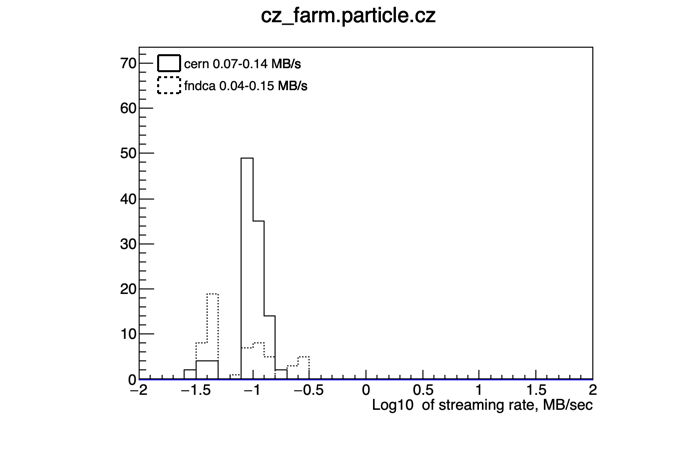
\includegraphics[width=0.45 \textwidth]{graphics/Workflow/dune_slow_2021_01_01_2021_04_30_0_cz_farm_particle_cz.png}
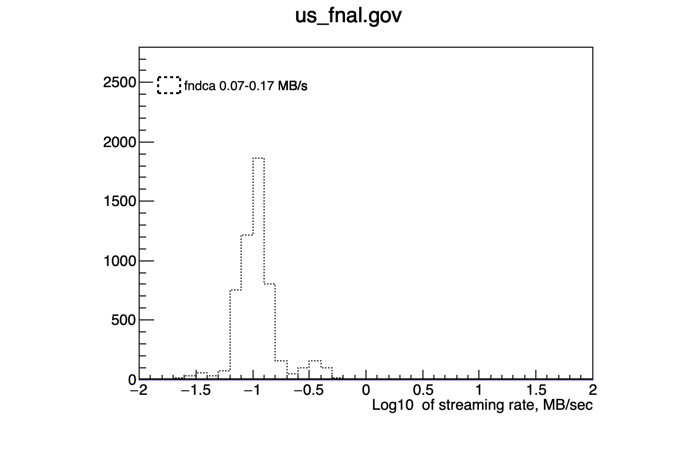
\includegraphics[width=0.45 \textwidth]{graphics/Workflow/dune_slow_2021_01_01_2021_04_30_0_us_fnal_gov.png}
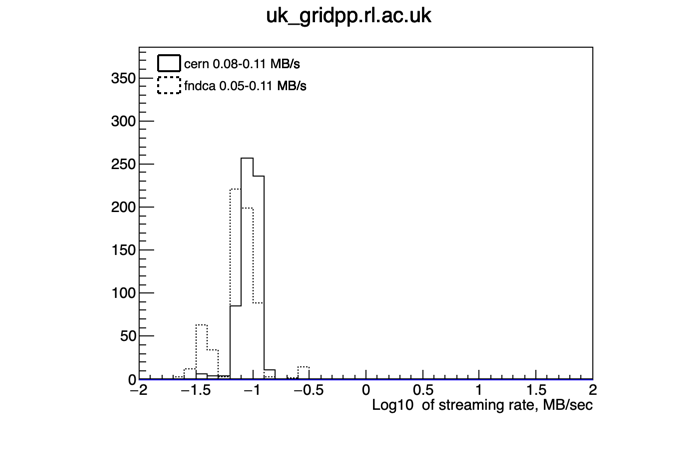
\includegraphics[width=0.45 \textwidth]{graphics/Workflow/dune_slow_2021_01_01_2021_04_30_0_uk_gridpp_rl_ac_uk.png}
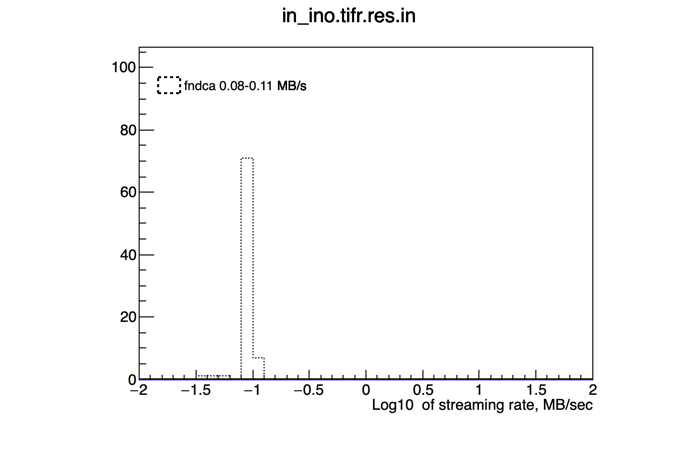
\includegraphics[width=0.45 \textwidth]{graphics/Workflow/dune_slow_2021_01_01_2021_04_30_0_in_ino_tifr_res_in.png}
\end{dunefigure}
%\todo{Get better figure}


\begin{dunefigure}
[Streaming speeds for tuple creation]
{fig:tuplespeed} 
{Streaming speeds for tuple creation jobs running at selected locations during a test in early January 2022. Reconstructed simulation files were located at sites in the UK and at Fermilab.  The histograms show the log10 of the inferred streaming rate (wall time/file size) for tuple creation jobs running at selected sites with different data sources.}
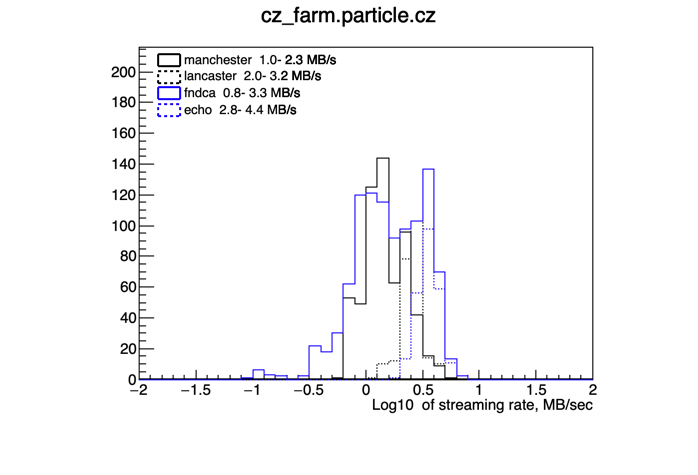
\includegraphics[width=0.45 \textwidth]{graphics/Workflow/dune_fast_2022_01_01_2022_01_07_0_cz_farm_particle_cz.png}
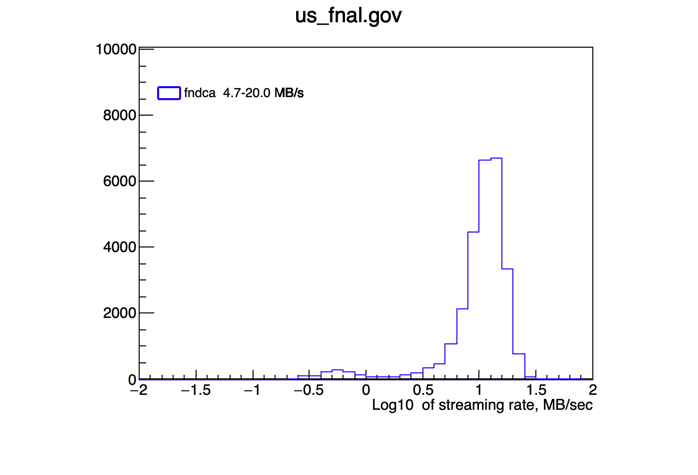
\includegraphics[width=0.45 \textwidth]{graphics/Workflow/dune_fast_2022_01_01_2022_01_07_0_us_fnal_gov.png}
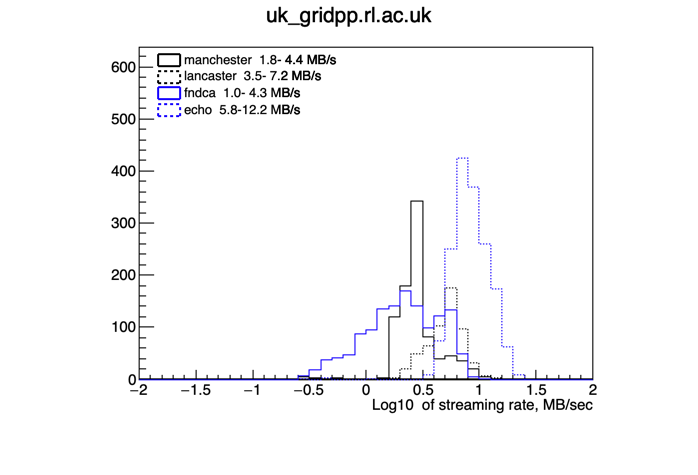
\includegraphics[width=0.45 \textwidth]{graphics/Workflow/dune_fast_2022_01_01_2022_01_07_0_uk_gridpp_rl_ac_uk.png}
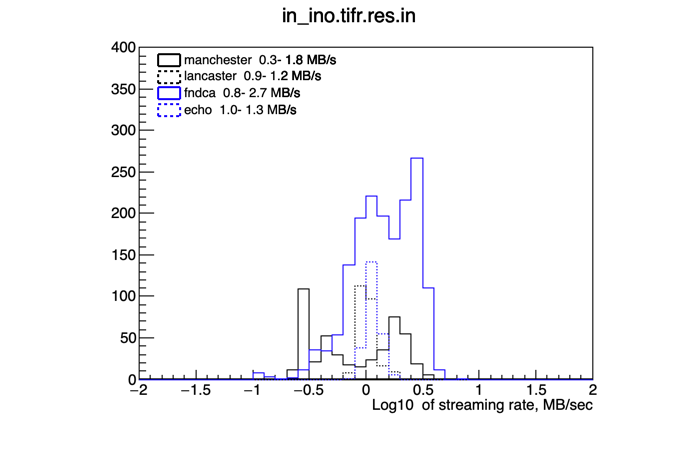
\includegraphics[width=0.45 \textwidth]{graphics/Workflow/dune_fast_2022_01_01_2022_01_07_0_in_ino_tifr_res_in.png}
\end{dunefigure}
%\todo{Get better figure}

\begin{dunefigure}
[Streaming speeds for tuple creation]
{fig:tuplespeedsummary} 
{Streaming speeds for tuple creation jobs running at multiple locations during a test in early January 2022. Reconstructed simulation was stored at sites in the UK and at Fermilab.  The average estimated streaming rates are plotted as a function of disk location ($x$-axis) and compute site ($y$-axis). Jobs in the US were required to use Fermilab disk but international sites were tested with multiple samples.}
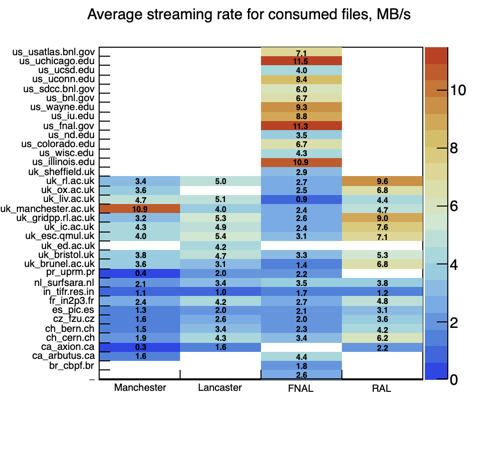
\includegraphics[width=0.8 \textwidth]{graphics/Workflow/fastRates.png}
\end{dunefigure}

\subsection{Implications for Data and Processing Placement}

The current study indicates that for CPU-dominated applications, notably reconstruction of raw data and simulation, the relative location of CPU resources is not critical. Wall time/MB   is similar regardless of location. For IO-dominated applications, proximity to the data is important.  Here there is a trade-off between the availability of resources and the efficiency with which they can be used. Intra-US processing, especially for locations near the national laboratories, is highly efficient, as is processing within the UK.  However, efficiency falls off as the CPU and disks become more separated.  

There are additional constraints imposed on our use of each site at scales greater than that of a single job. Due to local networking limitations, the number of jobs of a particular type we can run may need to be limited to avoid saturating the site's inbound or outbound capacity. 

We have the site information and monitoring tools to provide a workflow management system with the inputs it needs to do optimal placement of data and jobs to maximize efficiency. However our existing data management and workflow tools are not able to take full advantage of this information.  This motivates development of an improved workflow model described below and in Chapter~\ref{ch:wkflow}.



\section{Sites and Services \hideme{McNab - draft}}
\label{sec:cm:sites_and_services}  %% fix label according to section

% Some of this should goes to the Site Resources chapter 
% References to APIs and specific technologies
% perhaps even the definitions types of center and site too

The large \dword{lhc} experiments have historically relied on a tiered structure, with national Tier-1 centers % AM: serving -> and
and regional Tier-2 and Tier-3 centers.  The DUNE model builds on the emergence of faster networks to move to  a service-oriented model, where sites provide services, disk, CPU, real memory/core and archival tape, and projects are  distributed to them based on their capabilities and available networking.  For example, a site with large CPU and memory/core but slower networking would be ideal for simulation while small memory/core and fast access to large local disk stores would be ideal for high-level data analysis.  This model will require a high-level view of data locations and job placement with continual monitoring for bottlenecks, but allows new sites to contribute in an optimal way. The intent is to lower the bar for contributions without overburdening the core computing operations of the experiment.

This section sets out our ``Sites and Services'' model for using sites for DUNE computing tasks, including sites that participate in \dword{osg} or \dword{wlcg} more generally. Since our requirements are not the same as the \dword{lhc} experiments, this %necessitates a distinct naming scheme to 
requires implementing both a distinct naming scheme in
\dword{wlcg} and ways of mapping our scheme onto the \dword{wlcg} tier model.

At this stage, DUNE has chosen to express its requirements in terms of services provided by sites. Each site provides networking plus one or more approved DUNE services, which satisfy DUNE's minimum requirements for the service in terms of capacity, quality, and interfaces. This model allows us to avoid making assumptions about how sites and federations of sites will be organized in the future, as the community evolves away from the strict \dword{wlcg} tiers model towards \dword{doma} and concepts like %a
\dwords{datalake}.
%\todo{define data lakes please. Maybe add to glossary-comp-cdr. } %anne (already said) instead we express our requirements in terms of the services we interact with.

DUNE expects to be able to access services using broadly the same set of APIs as \dword{wlcg} (e.g., HTCondor-CE and \dword{xrootd}) and by using common cloud APIs (e.g., \dword{openstack} and \dword{s3}). 
%kirby - updated Mar 11 \todo{(anne) Should xroot be xrootd? I added the others to glossary-comp-cdr; please fill in the definitions}
For this reason, sites may be operated using conventional grid technologies, on-premises cloud systems, or commercial cloud services. Nevertheless, sites do appear in the DUNE computing model, as the atomic unit for operations activity. %Kirby - fixed Mar 11, 2022 \todo{(anne) This feels like a nonsequitur (and see ??? below)}
For example, staff at a site can receive and process tickets, %may  
and may be required to have a representative at an operations meeting with the technical knowledge to comment on issues as they arise.

In terms of workflows and data management, DUNE does not impose or require any hierarchy or grouping of sites, and assumes that, in general, data may flow between services at any two sites. That said, DUNE expects to use network proximity and bandwidth information to guide the efficient transfers of data between services. The details of the different services within the DUNE Computing Model are described in detail in Section~\ref{sec:cm:types_of_service}.

\section{Sites, Federations, and Countries\hideme{McNab - draft}}
\label{sec:cm:federations}

As well as sites, there are two more administrative concepts: federations and countries.
Federations are borrowed from \dword{wlcg} and represent one or more sites that together pledge a particular amount of capacity to DUNE and enter their pledges into a system like \dword{cric}. %Kirby commented it out since someone did this. \todo{add def to gloss}
Sites may choose to organize themselves this way as it allows more flexibility in how pledges are met against a background of planned upgrades at sites, unplanned outages, etc. 

Countries are represented directly or indirectly at the DUNE \dword{ccb}, and consist of one or more federations. Broadly, countries map to funding bodies and are 
the entity reviewed when evaluating the level of contribution to computing capacity relative to their number of DUNE members.   %Kirby - Mar 11, 2020 \todo{(anne) please clarify what's being compared, I don't get it. Where do you get number of members?} 




\section{Types of Service\hideme{McNab - draft}}
\label{sec:cm:types_of_service}

We envisage six classes of service on which we will put requirements and request capacity:

\begin{itemize}
    \item Network
    \item DUNE Computing Element
    \item Data Cache
    \item DUNE Storage Element
    \item DUNE Data Archive
    \item DUNE Analysis Facility
\end{itemize}

Note that each class of service may have varying levels or resources provided within a service, and the details of those levels are discussed in the following subsections.

\subsection{Network\hideme{McNab - draft}}
\label{sec:cm:network}

Networking is needed at all sites, with basic requirements including IPv4 and \dword{ipv6}. %Kirby someone did this \todo{please add to gloss, also NREN below}
All sites should be connected to the wide area network, typically via their \dword{nren}, with sufficient capacity to handle the data IO commensurate with their fraction of the workload. In practice this means at least 40\,Gbit/s for major sites with large amounts of storage (with 100\,Gbit/s becoming the normal expectation for a shared site such as a \dword{wlcg} Tier-1) and at least 20\,Gbit/s for smaller CPU-only sites (but with 40-100\,Gbit/s becoming the norm in shared sites).
Other DUNE-approved services may impose further requirements in terms of network capacity. %anne which they require,

\subsection{DUNE Computing Element\hideme{McNab - draft}}
\label{sec:cm:dce}

A DUNE Computing Element is a service that provides access to \dword{cpu} resources. % gives access to jobs consuming CPU. %anne  to perform computation. 
%anne To 
To minimize the operational overhead in working with 
each site, DUNE will require  minimum standards for:

\begin{itemize}
    \item The support level, in terms of whether tickets will be acted 24/7 or only during working hours
 %   the support level, in terms of whether tickets will be acted 24/7 or only during working hours
    \item the total number of logical processors across the service;
    \item the interface used to submit jobs or create virtual machines;
    \item the operating system version for grid capacity;
    \item memory and scratch disk space per processor;
    
    We note that DUNE computing, due to the large data objects, often requires a large memory footprint.  Provision of high memory  resources is very valuable.
    \item incoming and outgoing network capacity per processor; and
    \item %Suitable (already 'min standards for')
    access to a DUNE Storage Element or Data Cache, which allows data intensive jobs to execute without an unacceptably low CPU efficiency.
\end{itemize}

We envisage three subclasses within the computing element services aimed at centrally managed data processing, at user or working group data analysis, and at detector simulation, data cache, DUNE storage element, and DUNE data archive. These subclasses have different requirements for network access, and in the case of data analysis, for support level.

% HMS OK\todo{(anne) I'm taking these out of subsections -- too small.}
%\subsection{Data Cache\hideme{McNab - draft}}
%\label{sec:cm:data_cache}
The data cache, not managed by DUNE systems, requires:
\begin{itemize}
\item suitable networking,
\item sufficient nearby DUNE Compute Element capacity,
\item transparency, and
\item resiliency against transients to prevent jobs from dying and hence data loss.
\end{itemize}

%Suitable networking. Sufficient nearby DUNE Compute Element capacity to be useful. Not managed by DUNE systems. ``Transparent''. Data loss is equivalent to jobs dying, so a transient which DUNE systems will recover from.

%Kirby put this section back in because I think storage element is a first class service.
\subsection{DUNE Storage Element\hideme{McNab - draft}}
\label{sec:cm:dse}

The concept of a DUNE Storage Element mirrors that of a DUNE Compute Element. It must be of sufficient capacity, measured in hundreds of TB or in PB, for the operational overheard to be worthwhile. It must have a suitable support level. %defined above, in terms of whether tickets will be acted 24/7 or only during working hours. 
There must be enough inbound and outbound networking capacity for global data placement operations, and for jobs to write data there or to consume the data already present. In particular, there must be %anne
a minimum amount of DUNE Compute Element capacity available nearby, on which DUNE jobs can access 
 appropriate  storage services without   an unacceptably low CPU efficiency. For some jobs, for example full reconstruction and simulation, almost all storage services are appropriate while for analysis jobs, the only appropriate storage may be co-located at the same site. 
%while retaining sufficient CPU efficiency.

This formulation allows conventional grid sites with CPU and disk storage mixed together in adjacent racks, and also novel regional architectures such as data lakes %Kirby - done \todo{will be a gloss term!} %in which there is 
with sufficient network capacity to link CPU and storage at different locations. At this stage of the project, DUNE does not want to prejudge what will be available at the start of data taking, and does not want to discourage the exploration of new and more efficient ways of providing resources.


\subsection{DUNE Data Archive}
\label{subsec:data_archive}
Data archive is designed to be archival storage of \dword{dune} raw data, simulation, and any data derived from those files that must be permanently stored. Traditionally and as foreseen with \dword{dune}, this service has been provided by tape storage facilities. There are currently at least five institutions providing tape storage facilities with the largest and most important providers being FNAL and CERN. The volume and access patterns for these services is an ongoing area of research and development to both keep up with modern technology and to understand how it impacts \dword{dune}'s ability to accomplish physics.

\subsection{DUNE Analysis Facility}

Most data analysis is currently being done using serial reads of \dword{larsoft} outputs or small root ntuples.  DUNE is actively exploring dedicated analysis facilities capable of columnar access to data and more sophisticated analysis techniques and notebook based analysis. 


\subsubsection{Coffea framework}
 
\subsubsection{Compute Canada Prototype}

An interactive analysis facility has been prototyped on a cloud allocation provided by Compute Canada’s OpenStack platform on the Arbutus Cloud (https://docs.computecanada.ca/wiki/Cloud\_resources). This experimental allocation is dedicated to DUNE and currently includes 300 virtual CPUs, 2.2 TB of shared memory, 2 TB disk storage, and 1 TB of CephFS storage that uses a shared storage protocol. More storage has been requested for the next resource allocation year (2022). 

Several computing nodes, each with 8 CPUs and 90 GB of memory, have been formed out of this allocation. The facility relies on Jupyterhub to implement a web-based interactive experience and uses containerization technologies to maintain a dedicated workspace for each authenticated user. Kubernetes is the industry-standard platform for this use case and can be deployed at scale for up to 5000 nodes (https://kubernetes.io/docs/setup/best-practices/cluster-large/). User authenticates through CILogon and a single-user JupyterLab server on a Scientific Linux 7 Docker image is quickly deployed thereafter. 

The facility provides a few features to facilitate analysis. Larsoft and DUNE-specific libraries are enabled through CVMFS trivially. Users building event loop-based analysis routines will have the identical experience to the bash-based virtual machines. Data files can be streamed with xrootd once users authenticate with the VOMS server. 

Coffea (https://coffeateam.github.io/) is a new analysis framework that could enable analyses on the fly with a quick turnaround time and a low barrier for a new analyzer. The framework was originally developed by LHC collaborators to enable columnar-based analyses of large volumes of LHC data in flat ROOT format using Python. Coffea employs uproot for file I/O and uses a NanoEvent class to parse TTree branches into user-defined physics objects for columnar computation. Users have the option to distribute their computations across different CPUs using a Dask (https://dask.org/) cluster. 

A prototype NanoEvent for the ProtoDUNE PDSPAnalyzer flat analysis format is already available with the goal of demonstrating a full-chain analysis (event selection, background tuning, systematics). Small scale test of data streaming from FNAL using xrootd has also been successful. 

Longer-term goals include migrating the facility to a managed service provided by Arbutus, investigating token-based authentication to seamless bridge user login and grid authorization, understanding network limitations and means to circumvent them. 

\subsubsection{Analysis Facility Issues}
One of the major issues for a dedicated analysis facility is the ability to access and maintain data samples.  We expect that, with many different analysis users, many disparate data samples will need to be available at any given facility but they must also be on local storage to maintain optimal efficiency.

%\subsection{DUNE Data Archive\hideme{McNab - needs work}}

%Kirby - just not really need this sentence. Networking. Cache? Support level? Tape without saying only tape forever. \todo{Anne ignored this!}

%The host laboratory is the most important center and during DUNE data %taking will be FNAL. During protoDUNE data taking, both FNAL and CERN %have host laboratory roles. A host laboratory runs central services %for DUNE, makes the largest single contribution in disk and CPU, and %acts as an archive center and user center. This broadly corresponds %to the WLCG Tier-0 concept. 
%
%Archive centers fulfill DUNE’s requirement to have two copies of raw %data on tape (or other archival-quality storage systems), including %one not at the Host Laboratory. It is not essential that archive %centers also have significant amounts of disk and CPU available to %DUNE as they may only be needed for disaster recovery and for %recovering individual lost files. Amongst WLCG sites, archive centers %would be based on the tape archives of Tier-1s, and the concept maps %directly to the DOMA idea of an archive center where disk storage and %CPU may be absent.
%
%Disk centers provide storage managed by DUNE, along with significant %amounts of CPU, and satisfy DUNE’s requirements for the ratio of CPU %to disk, the bandwidth between CPU and disk, and the bandwidth to and %from other participating centers. DUNE does not require 24/7 on call %support for disk centers, but may use the declared support level when %deciding where to place data and where to direct workflows. Disk %centers correspond to WLCG Tier-1 sites or Tier-2 sites with disk, %and to DOMA Data and Compute Centers.
%
%Compute centers provide only CPU capacity, scratch disk associated %with jobs running on worker nodes for the duration of jobs, and %possibly transparent caching (eg Xcache). That is, they do not %provide storage which is managed by DUNE. They do however satisfy %DUNE’s requirements for bandwidth to and from other participating %centers. Compute centers correspond to WLCG Tier-2 sites without %disk, and to DOMA compute centers. 
%
%User centers are used for end user analysis, by people submitting %jobs and managing workflows, and may need to download or stream a %limited amount of data directly from disk centers.
%
%
%
%\section{Requirements for Computing Services \hideme{McNab - needs %work}}
%
%What we need DUNE services to be able to do, to do the above.
%
%
%\todo{consider both cases of data to job and job to data - discuss %current issues but be vague about the future}
%
%%%%%%%%%%% notes from 10-29

% Define a minimal "CPU-only" service

% Define a DUNE-managed disk service - how many TB min - requires support. 

% Define a tape service

% Mention possible need for cache for 

%(How do they get the code? cvmfs or container.  

%\todo{Andrew compares the use case footprint table into a sites %comparison}
\end{document}